\subsection{Drivetrain}\label{Drivetrain}
The drivetrain translates the torque $\tau_m$, given by the motor, into the actual movement of the vehicle. The model of the drivetrain illustrates the relation between the applied torque, $\tau_m$, and the velocity of the vehicle. The velocity model of the drivetrain is created by only considering when the vehicle's trajectory follows a straight line.\\\\
%
The modeling of the drivetrain is limited to only modeling parts of the total drivetrain system, to make it more manageable and with a focus on giving a rough approximation.

\subsubsection{Model of the Internal Gears}\label{BlackBoxModel}
To get a rough approximation of the effect of the drivetrain, a black boxed model is used. The black box in the model is placed between box 1 and including box 3 seen in \chapref{sec:Vehicledescription} \figref{vehicleDescriptionDriveTrain}. The gear, $G_m$, connected to the motor shaft, is connected to the gear, $G_d$, which represents the gears and shafts that has been black boxed, where the output appears on the shaft connected to the drive-wheel, $G_t$, see \figref{fig:DrivetrainMechanicalModel}. The number of teeth on the gear, $G_d$, represents the ratios throughout the drivetrain, such that the gear ratio between $G_m$ and the output at the drive gear is given by: $\frac{N_m}{N_d}$, where $N_m$ is the number of teeth on the motor gear and $N_d$ is the calculated number of teeth on the black box gear.

\begin{figure}[H]
	\centering
	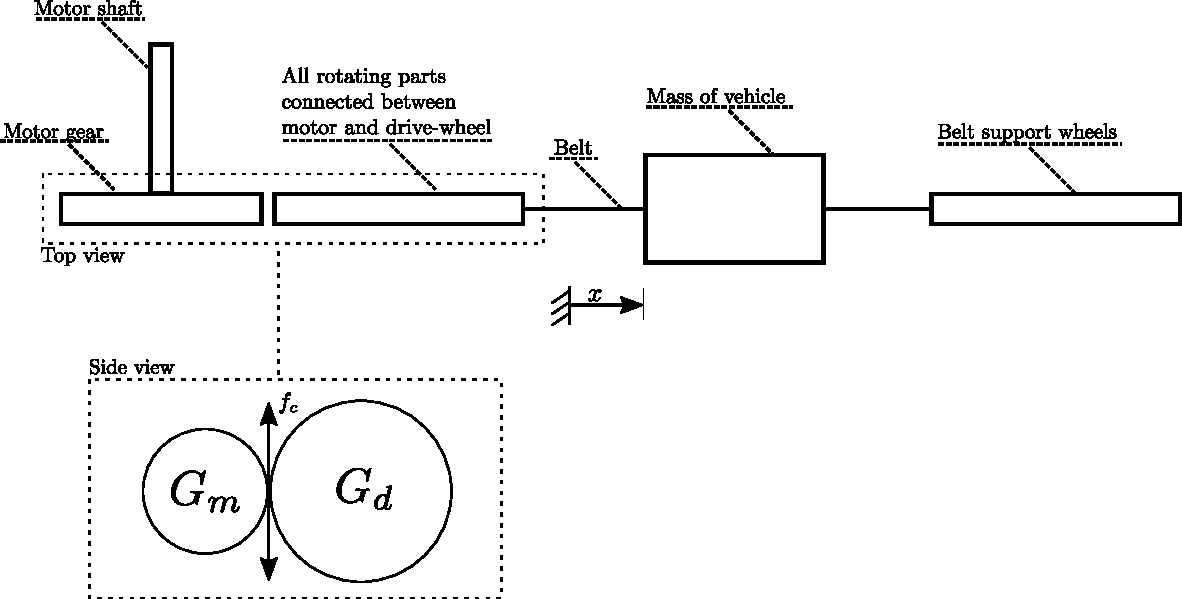
\includegraphics[scale=0.8]{figures/mechanicalDrawingSystem.pdf}
	\caption{A diagram showing the rough mechanical model of the drivetrain}
	\label{fig:DrivetrainMechanicalModel}
\end{figure}

The torque of the motor along with the contributions from the load, i.e. the drivetrain, affecting the motor shaft, is depicted in as a free body diagram in \figref{fig:MotorGearFreeBodyDiagram}.

\begin{figure}[H]
	\centering
	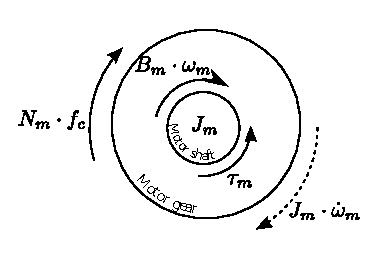
\includegraphics[scale=1.2]{figures/freeBodyMotorGear.pdf}
	\caption{A free body diagram of the motor gear, $G_m$}
	\label{fig:MotorGearFreeBodyDiagram}
\end{figure}

The radius of the motor gear times the contact force, $r_d \cdot f_c$, is the torque translated from the motor gear, $G_m$, to the gear representing the drivetrain, $G_d$, in \figref{fig:BlackBoxGearFreeBodyDiagram}. Thus it appears as an opposing torque to the applied motor torque, $\tau_t$. From \figref{fig:MotorGearFreeBodyDiagram}, the following equation can be derived:
 \begin{flalign}
   \eq{J_m \cdot \dot{\omega}_m(t)} {\tau_m(t) - B_m \cdot \omega_m(t) - r_m \cdot f_c(t)}\unit{N \cdot m}\nonumber
   \label{eq:MotorGearNewtonSecLaw}
 \end{flalign}
%
\hspace{6mm} Where:\\
\begin{tabular}{ p{1cm} l l l}
& $J_m$ 						& is the motor's inertia                                         &\unitWh{kg \cdot m^2} \\
& $\omega_m$        & is the angular velocity of the motor                           &\unitWh{rad \cdot s^{-1}} \\
& $\dot{\omega}_m$ 	& is the angular acceleration of the motor                       &\unitWh{rad \cdot s^{-2}} \\
& $\tau_m$ 			    & is the torque delivered by the motor                           &\unitWh{N \cdot m} \\
& $B_m$             & is the motor's friction coefficient                            &\unitWh{N \cdot m \cdot s \cdot rad^{-1}} \\
& $r_m$             & is the radius of the gear, $G_m$, connected to the motor shaft &\unitWh{m} \\
& $f_c$							& is the contact force between the two gears                     &\unitWh{N}
\end{tabular}

To describe the translations of the torques throughout the system an other free body diagram is applied in \figref{fig:BlackBoxGearFreeBodyDiagram}, showing the system's effects on the blackbox gear, $G_d$, giving the output on the drive gear.

\begin{figure}[H]
	\centering
	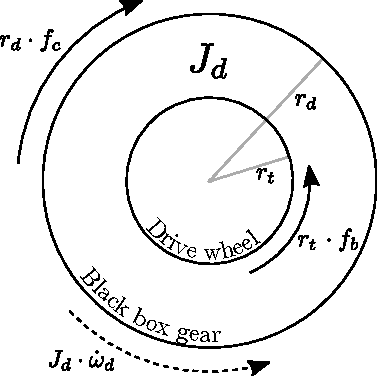
\includegraphics[scale=1]{figures/freeBodyDriveGear.pdf}
	\caption{A free body diagram of the `black box' gear, $G_d$}
	\label{fig:BlackBoxGearFreeBodyDiagram}
\end{figure}

An equation is extracted from \figref{fig:BlackBoxGearFreeBodyDiagram}:
\begin{flalign}
\eq{J_d \cdot \dot{\omega}_d(t)}{r_d \cdot f_c(t) - r_t \cdot f_b(t)} \unit{N\cdot m}
\label{eq:BlackBoxGearNewtonSecLaw1}
\end{flalign}
\hspace{6mm} Where:\\
\begin{tabular}{p{1cm}lll}
& $J_d$ 						& is the `black box' gear inertia                                    &\unitWh{kg \cdot m^2} \\
& $\dot{\omega}_d$ 	& is the angular acceleration of the `black box' gear, $G_d$         &\unitWh{rad \cdot s^{-2}} \\
& $r_d$             & is the radius of the `black box' gear, $G_d$                       &\unitWh{m} \\
& $r_t$             & is the radius of the drive wheel, $G_t$ (translational)            &\unitWh{m} \\
& $f_b$             & is the coefficient of the contact force between $G_d$ and the belt &\unitWh{N} \\
& $f_c$						  & is the contact force between the two gears                         &\unitWh{N}
\end{tabular}

Two equations for the internal gears have been found, \eqref{eq:MotorGearNewtonSecLaw} and \eqref{eq:BlackBoxGearNewtonSecLaw}. In the following paragraph a model of the translation between the drive-gear and the belt will be created.

%% SSSECTION : BELT MODEL %%
\subsubsection{Model of the Vehicle's acceleration}\label{BeltModel}
It is necessary to find the translation between the drive-gear and the belt to be able to describe the movement of the vehicle. Furthermore, it is needed to be able to make a full model of the system, going from the gear connected to the motor shaft to the vehicle's belts. In \figref{fig:BeltMechanicalDiagram} a mechanical diagram illustrates how the force given through the drive wheel is translated by the belts to a linear force acting on the mass which in turn yields the vehicle's velocity.

\begin{figure}[H]
	\centering
	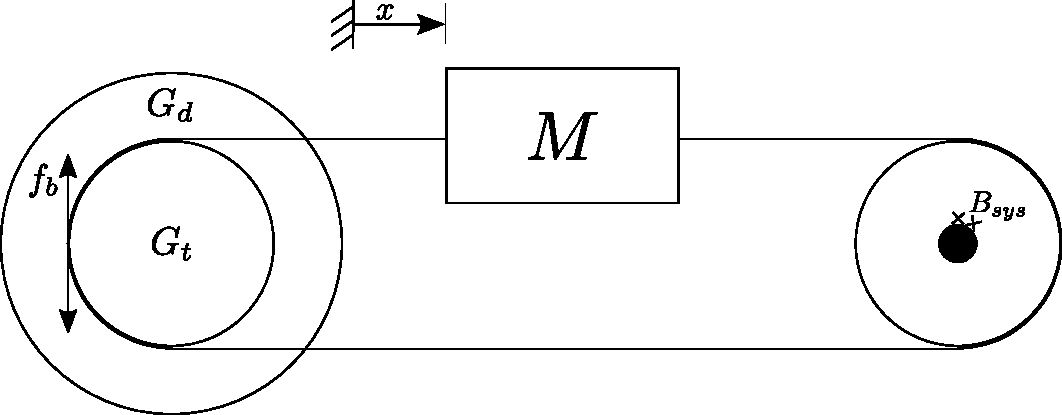
\includegraphics[scale=0.8]{figures/mechanicalDrawingBelt.pdf}
	\caption{A mechanical diagram of the drive-gear rotating the belt affected by the vehicle's mass}
	\label{fig:BeltMechanicalDiagram}
\end{figure}

By using \figref{fig:BeltMechanicalDiagram} a free body diagram of the mass, $M$, and the forces applied to it is derived.

\begin{figure}[H]
	\centering
	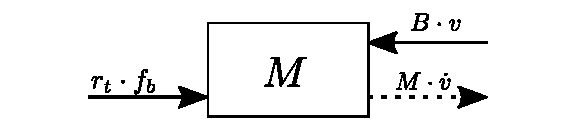
\includegraphics[scale=.8]{figures/freeBodyBelt.pdf}
	\caption{A free body diagram illustrating the vehicle's mass affected by the surrounding forces}
	\label{fig:BeltFreeBodyDiagram}
\end{figure}

From \figref{fig:BeltFreeBodyDiagram}, a mechanical equation of the vehicle's resulting force is found to be:\todo{In free body diagram: remove rt, the forces should be in N, not N*m}
%
\begin{flalign}
\eq{M \cdot \dot{v}(t)}{f_b(t) - B_{sys} \cdot v(t)} \unit{N}
\label{eq:BeltMassNewtonSecLaw}
\end{flalign}
\hspace{6mm} Where:\\
\begin{tabular}{p{1cm}lll}
& $M$ 			  & is the vehicle's total weight                                        &\unitWh{kg} \\
& $v$        	& is the linear velocity of the vehicle                                &\unitWh{m \cdot s^{-1}} \\
& $\dot{v}$ 	& is the linear acceleration of the vehicle                            &\unitWh{m \cdot s^{-2}} \\
& $B_{sys}$   & is the coefficient of the friction throughout the rotational parts   &\unitWh{N \cdot s \cdot m^{-1}} \\
\end{tabular}

In the following section the three mechanical equations, \eqref{eq:MotorGearNewtonSecLaw}, \eqref{eq:BlackBoxGearNewtonSecLaw1} and \eqref{eq:BeltMassNewtonSecLaw} will be combined.

\subsubsection{Model of the Combined Drivetrain}\label{DrivetrainModeling}
In this section a model will be created of the combined drivetrain, by assembling the derived mechanical equations, \eqref{eq:MotorGearNewtonSecLaw}, \eqref{eq:BlackBoxGearNewtonSecLaw1} and \eqref{eq:BeltMassNewtonSecLaw}. This allows to get a linear velocity of the vehicle, $v$, from the torque, $\tau_m$, delivered by the motor. The three equations are linked through the contact forces $f_c$ and $f_b$.\\\\
%
The Laplace-transform is applied on the three equations in order to be able to deduce a transfer function of the input torque, $\tau_m(s)$, to the output velocity, $V(s)$:
%
\begin{flalign}
\eq{J_m \cdot \omega_m(s) \cdot s}{\tau_m(s) - B_m \cdot \omega_m(s) - r_m \cdot F_c(s)}&
\label{eq:MotorGearNewtonSecLawLaplace}
\end{flalign}
%
\begin{flalign}
\eq{J_d \cdot \omega_d(s) \cdot s}{r_d \cdot F_c(s) - r_t \cdot F_b(s)}&
\label{eq:BlackBoxGearNewtonSecLawLaplace}
\end{flalign}
%
\begin{flalign}
\eq{M \cdot V(s) \cdot s}{F_b(s) - B_{sys} \cdot V(s)}&
\label{eq:BeltMassNewtonSecLawLaplace}
\end{flalign}

$F_c$ is isolated from \eqref{eq:MotorGearNewtonSecLawLaplace}:
\begin{flalign}
\eq{F_c(s)}{\frac{\tau_m(s) - B_m \cdot \omega_m(s) - J_m \cdot \omega_m(s) \cdot s}{r_m}}&
\label{eq:GearsContactForceMotorGearLaplace}
\end{flalign}
%
$F_b$ is isolated from \eqref{eq:BlackBoxGearNewtonSecLawLaplace}:
\begin{flalign}
\eq{F_b(s)}{\frac{r_d \cdot F_c(s) - J_d \cdot \omega_d(s) \cdot s}{r_t}}&
\label{eq:GearsContactForceBlackBoxGearLaplace}
\end{flalign}
%
$F_b(s)$ is isolated from \eqref{eq:BeltMassNewtonSecLawLaplace}.
\begin{flalign}
\eq{F_b(s)}{V(s) \cdot (M \cdot s - B_{sys})}&
\label{eq:BeltContactForceLaplace}
\end{flalign}

The $F_c(s)$ in \eqref{eq:GearsContactForceBlackBoxGearLaplace} is substituted for the expression given by \eqref{eq:GearsContactForceMotorGearLaplace}:
\begin{flalign}
\eq{F_b(s)}{\frac{r_d \cdot (\frac{\tau_m(s) - B_m \cdot \omega_m(s) - J_m \cdot \omega_m(s) \cdot s}{r_m}) - J_d \cdot \omega_d(s) \cdot s}{r_t}}&\nonumber\\
\eq{F_b(s)}{\frac{\tau_m(s) \cdot r_d}{r_m\cdot r_t} - \frac{\omega_m(s)\cdot r_d}{r_m\cdot r_t}\cdot (B_m + J_m \cdot s) - \frac{\omega_d(s)}{r_t}\cdot J_d\cdot s}&
\label{eq:BlackBoxGearNewtonSecLawLaplace&MotorGearNewtonSecLawLaplace}
\end{flalign}

The two expressions for $F_b(s)$ in \eqref{eq:BlackBoxGearNewtonSecLawLaplace&MotorGearNewtonSecLawLaplace} and \eqref{eq:BeltContactForceLaplace} respectively are coupled:
\begin{flalign}
\eq{V(s) \cdot (M \cdot s - B_{sys})}{\frac{\tau_m(s) \cdot r_d}{r_m\cdot r_t} - \frac{\omega_m(s)\cdot r_d}{r_m\cdot r_t}\cdot (B_m + J_m \cdot s) - \frac{\omega_d(s)}{r_t}\cdot J_d\cdot s}&
\label{eq:BlackBoxGearNewtonSecLawLaplace&MotorGearNewtonSecLawLaplace&&BeltContactForceLaplace}
\end{flalign}

Converting all rotational velocities to linear velocities through use of the relation of ratios:
\begin{flalign}
\eq{\frac{r_m}{r_d}}{\frac{\omega_d(t)}{\omega_m(t)}}\nonumber \unit{\cdot}\\
\eq{\omega_d(t)}{\frac{r_m}{r_d}\cdot \omega_m(t)} \unit{rad\cdot s^{-1}}
\label{eq:ratioes}
\end{flalign}

Converting $\omega_d(t)$ to linear velocity and transforming to Laplace domain:
\begin{flalign}
\eq{v(t)}{\omega_d(t) \cdot 2 \cdot \pi \cdot r_t}\nonumber \unit{m\cdot s^{-1}} \phantom{(3.23   3)}\\
\eq{\omega_d(t)}{\frac{v(t)}{2\cdot \pi \cdot r_t}} \ \xRightarrow{\mathcal{L}} \ \omega_d(s) = \frac{V(s)}{2\cdot \pi \cdot r_t}&
\label{eq:omegaDtoLinearLaplace}
\end{flalign}

Converting $\omega_m(t)$ to linear velocity using \eqref{ratioes} and \eqref{omegaDtoLinearLaplace} and transforming to Laplace domain
\begin{flalign}
\eq{\frac{r_m}{r_d}\cdot \omega_m(t)}{\frac{v(t)}{2\cdot \pi \cdot r_t}}\nonumber \unit{rad\cdot s^{-1}} \phantom{(3.23   3)}\\
\eq{\omega_m(t)}{\frac{v(t)\cdot r_d}{2\cdot \pi \cdot r_t\cdot r_m}}  \ \xRightarrow{\mathcal{L}} \ \omega_m(s) = \frac{V(s)\cdot r_d}{2\cdot \pi \cdot r_t\cdot r_m}
\label{eq:omegaTtoLinearLaplace}
\end{flalign}



%-------------------------------------Niels corrected to here-------------------------------------------------------------




The $\omega_d$ and $F_b$ in \eqref{eq:GearsContactForceLaplace} are replaced:
\begin{flalign}
\eq{F_c(s)}{\frac{J_d \cdot s}{N_d} \cdot \frac{1}{r_t} \cdot V(s) + V(s) \cdot \left[\frac{M \cdot s + B_{tot}}{r_t}\right]} \unit{unit}\\
\eq{F_c(s)}{V(s) \cdot \left[\frac{J_d \cdot s}{r_t \cdot N_d} + \frac{M \cdot s + B_{tot}}{r_t} \right]} \unit{unit}
\label{eq:GearsContactForceLaplaceNew}
\end{flalign}

The desired relation between the motor torque and the linear velocity is obtained:
\begin{flalign}
\eq{\tau_m(s)}{J_m \cdot \frac{N_d}{N_m \cdot r_t} \cdot V(s) \cdot s + B_m \cdot \frac{N_d}{N_m \cdot r_t} \cdot V(s) + N_m \cdot \left[\frac{J_d \cdot s}{r_t \cdot N_d} + \frac{M \cdot s + B_{tot}}{r_t} \right] \cdot V(s)} \unit{unit}
\end{flalign}
\begin{flalign}
\eq{\tau_m}{V(s) \cdot \frac{1}{r_t} \cdot \left[\frac{J_m \cdot N_d}{N_m} \cdot s + N_m \cdot J_d \cdot s + M \cdot s + N_m \cdot B_{tot} + B_m \cdot \frac{N_d}{N_m} \right]} \unit{unit}
\end{flalign}

The transfer function with the relation between the input torque, $\tau_m$, and the output velocity, $V$, given by:
\begin{flalign}
\eq{\frac{V(s)}{\tau_m(s)}}{\frac{r_t}{\left[\frac{J_m \cdot N_d}{N_m} + N_m \cdot J_d + M\right] \cdot s + \left[B_{tot} \cdot N_m + B_m \cdot \frac{N_d}{N_m} \right]}} \unit{unit}
\label{eq:TransferFunctionTorqueToVelocity}
\end{flalign}

It is possible to draw a block diagram for the drivetrain, from the motor torque to the vehicle's velocity with \eqref{eq:TransferFunctionTorqueToVelocity}. Furthermore, the motor needs the produced angular velocity to get affected by the load, i.e. drivetrain. The angular velocity was found in \eqref{eq:BlackBoxGearNewtonLaplaceNew}.

\begin{figure}[H]
	\centering
	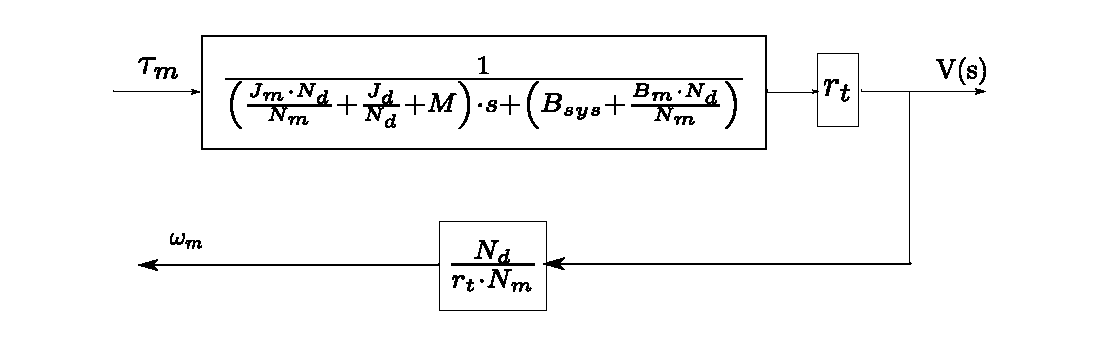
\includegraphics[scale=1]{figures/blockDiagramDrivetrain.pdf}
	\caption{A block diagram of the combined drivetrain}
	\label{fig:BlockDiagramDrivetrain}
\end{figure}

A block diagram describing the drivetrain has been built. In the following section the drivetrain's block diagram is combined with the motor's block diagram, seen in \figref{fig:motormodelBlock}.